\documentclass[../../ASSD_TP1_G7.tex]{subfiles}
\begin{document}
\chapter*{Remuestreo}
Para realizar la medición se utiliza el sample and hold y la llave analógica en contra fase, es decir la se\~nal de control de la llave y el sample and hold son inversas. Permitiendo lograr un muestreo similar al instantáneo, ya que la se\~nal es constante en el momento que la llave analógica se acciona.

La se\~nal se puede describir matemáticamente de la siguiente manera:

\begin{equation}
x_{s}(t)=\left[ x(t)\left( \sum_{i=-\infty}^{\infty} \delta(t - i T_s) \right) \right]* \pi(\frac{t}{\tau})
\end{equation}

\par Donde $x(t)$ se\~nal antes y $x_{s}(t)$ es la se\~nal después de la llave analógica y el sample and hold.$T_s$ es el periodo de sampleo y $\tau$ es el ancho de la ventana del sample and hold.
\par Aplicando la transformada de Fourier a la esxpresion de $x_{s}$ se obtiene su espectro.

\begin{equation}
X_{s}(f)=\left( \sum_{k=-\infty}^{\infty} X(f - k f _s) \right) f _s \tau sinc(f \tau) \label{eq:espectroRemuestreo}
\end{equation}

Tal como se observa en la ecuación \ref{eq:espectroRemuestreo}, el espectro de la se\~nal esta deformado por un sinc. Par solucionar este problema, una opción seria agrandar el $\tau$, el sinc tendería a la delta, pero se produce una perdida de potencia. Otra opción es achicar el $\tau$ , el ancho del sinc aumenta, el problema es comienzan aparecer repeticiones del espectro que antes se encontraban atenuadas por el sinc, produciendo aliasing.



\section*{Mediciones}

Las mediciones se efectuaron con la siguiente se\~nal AM:

\begin{equation}
X_c=A_{Max}[\frac{1}{2}cos(2\pi (1.8 f_{in})t)+cos(2\pi (2 f_{in})t)+cos(2\pi (2.2 f_{in})t)]
\end{equation}\label{eq:inputSignlanAM}

Donde $f_{in}=45KHz$.

\subsection*{Sample and hold}
Se utilizo un duty cycle de 40\% y una frecuencia se sampleo de 100KHz.
\begin{figure}[H]
\centering
\subcaptionbox{Simulacion}
{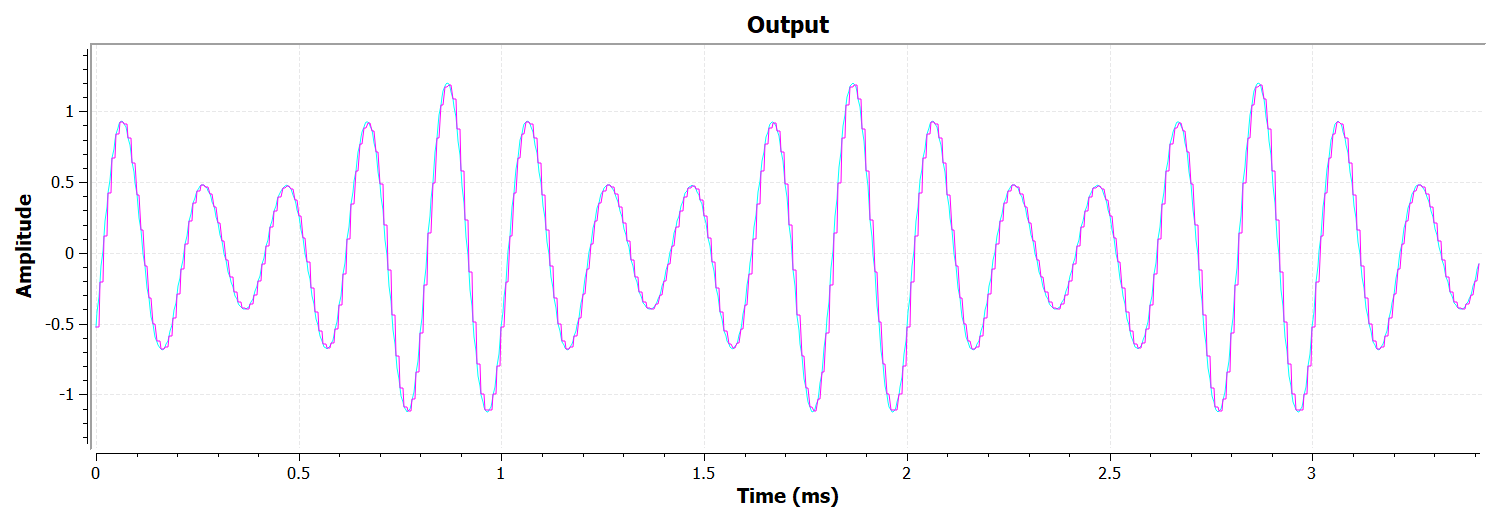
\includegraphics[width=0.5\textwidth]{figures/simsyh_pto_7_4.png}}
\subcaptionbox{Medicion}
{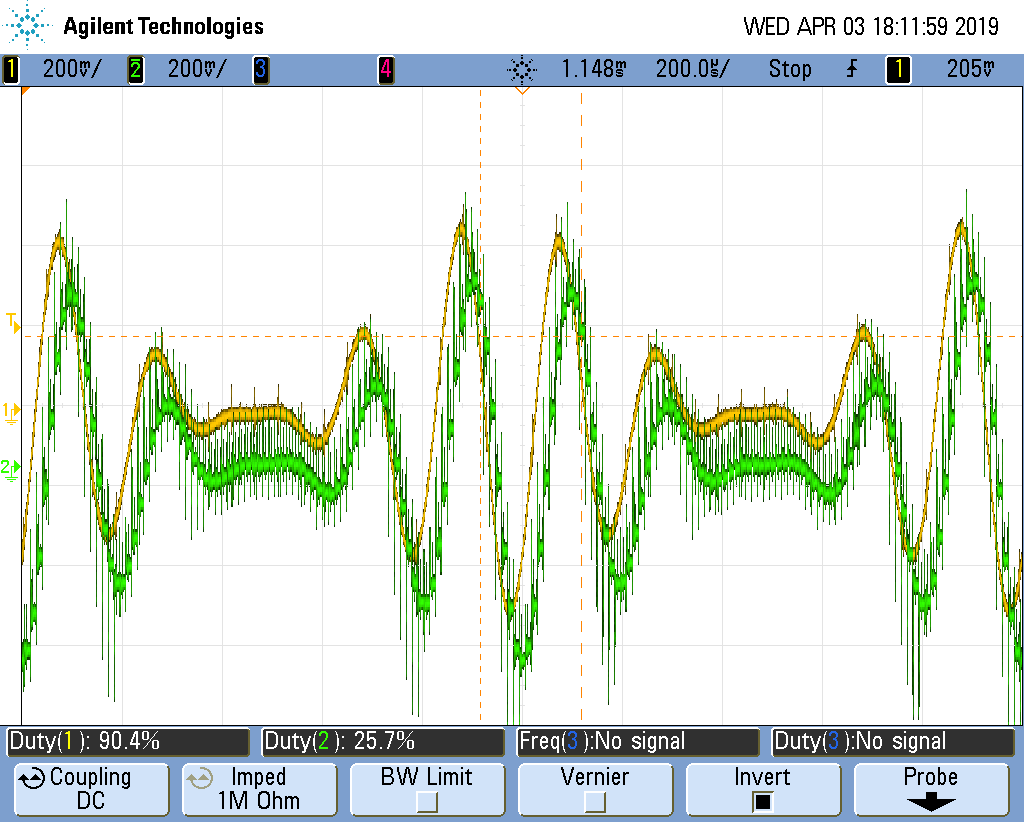
\includegraphics[width=0.45\textwidth]{figures/syh_pto_7_4.png}}
\caption{Remuestreo de la se\~nal con sample and hold}
\end{figure}

\begin{figure}[H]
\centering
\subcaptionbox{Simulacion}
{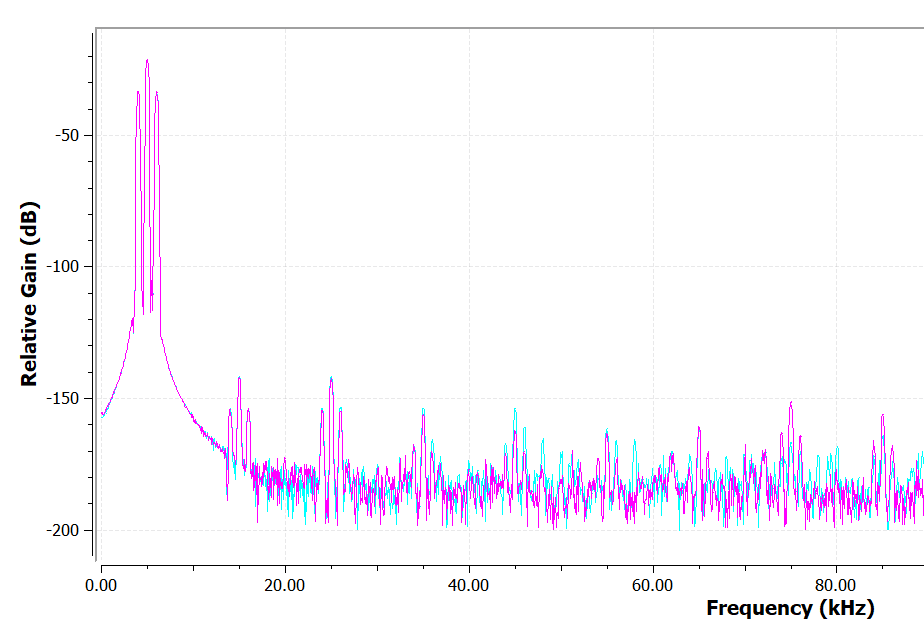
\includegraphics[width=0.5\textwidth]{figures/simespectosyh.PNG}}
\subcaptionbox{Medicion}
{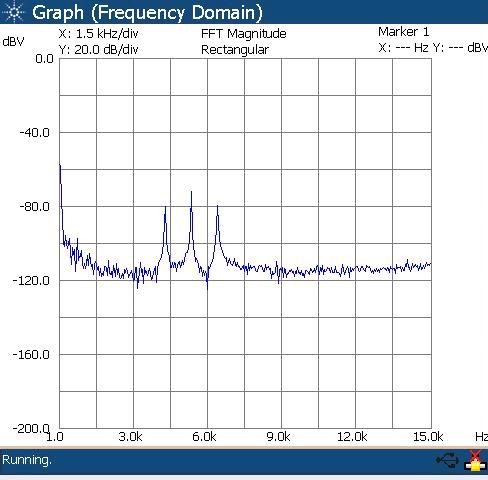
\includegraphics[width=0.45\textwidth]{figures/syh.jpeg}}
\caption{Espectro de la se\~nal despues del sample and hold}
\end{figure}



\subsection*{Sample and hold y llave analógica, sin filtro recuperador}
\begin{figure}[H]
\centering
\subcaptionbox{Simulacion}
{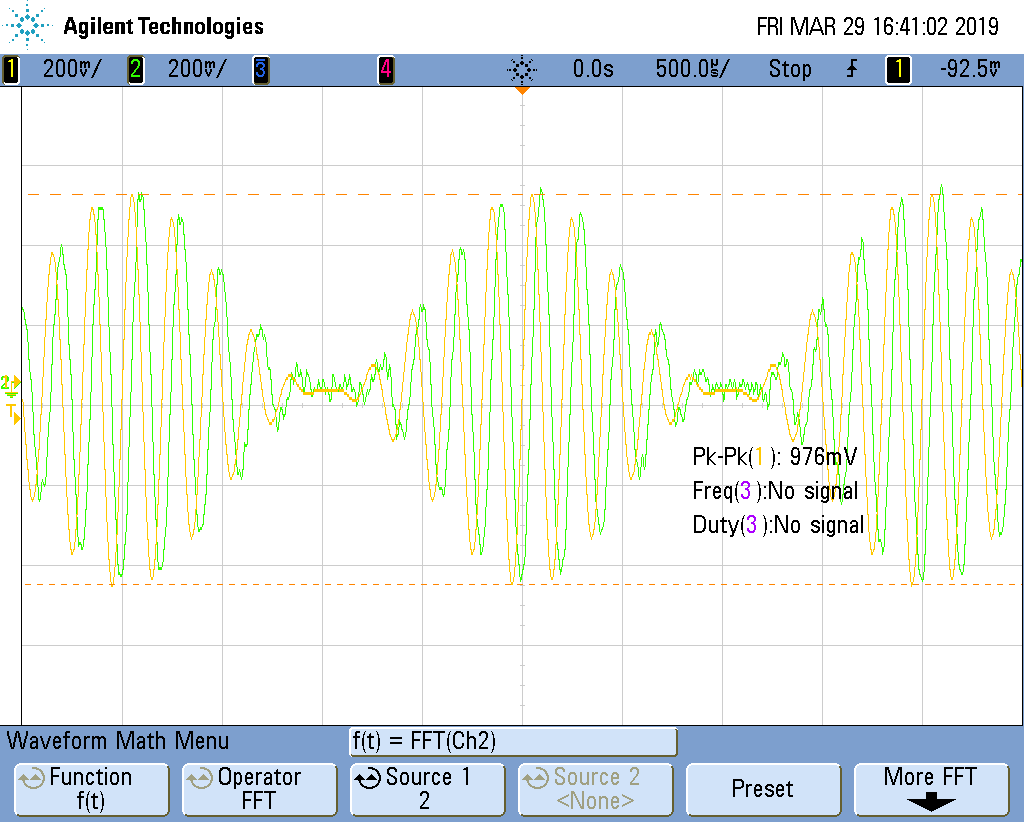
\includegraphics[width=0.45\textwidth]{figures/syh_ptp_7re.png}}
\subcaptionbox{Medicion}
{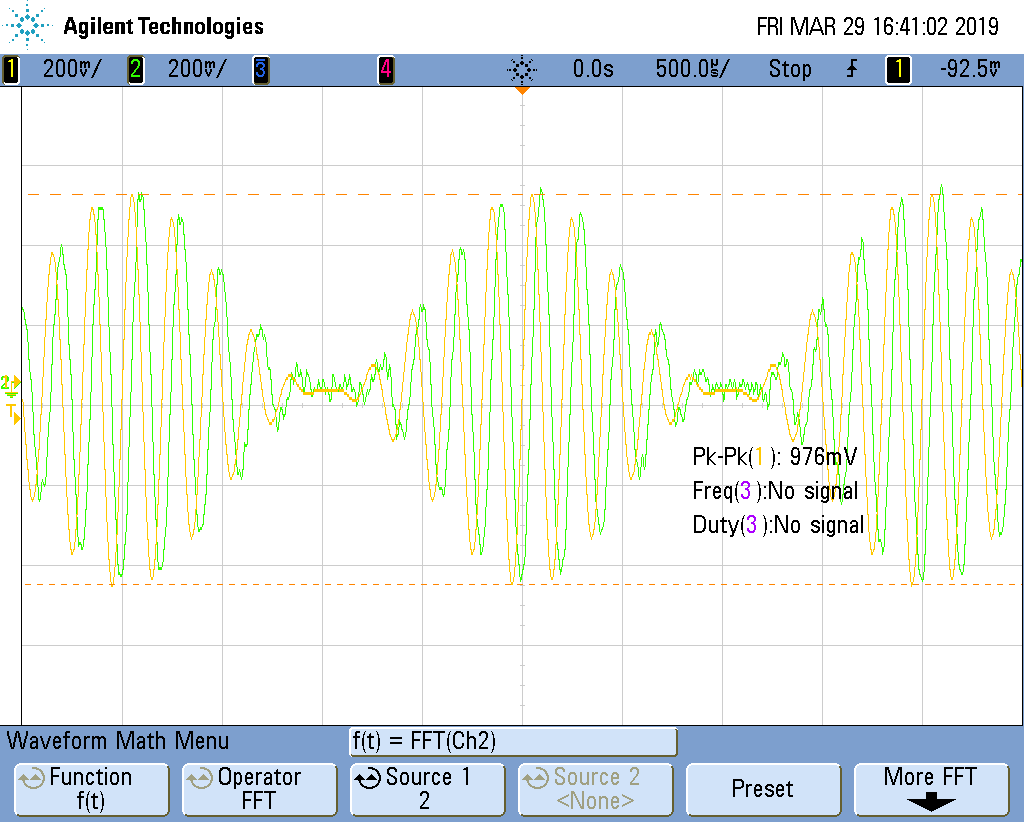
\includegraphics[width=0.45\textwidth]{figures/syh_ptp_7re.png}}
\caption{Remuestreo de la se\~nal con sample and hold y llave analógica}
\end{figure}

\subsection*{Sample and hold y llave analógica, con filtro recuperador}
\begin{figure}[H]
\centering
\subcaptionbox{Simulacion}
{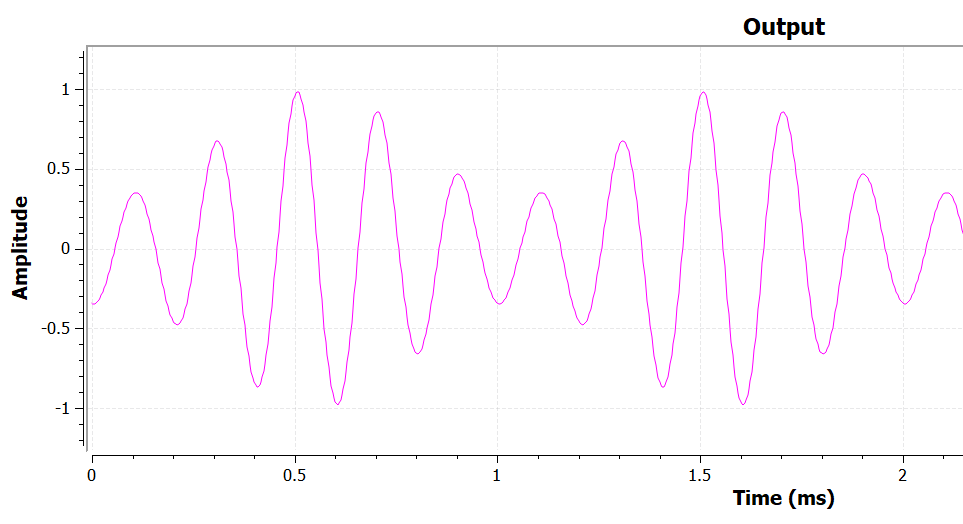
\includegraphics[width=0.45\textwidth]{figures/simlyh_pto_7_3.png}}
\subcaptionbox{Medicion}
{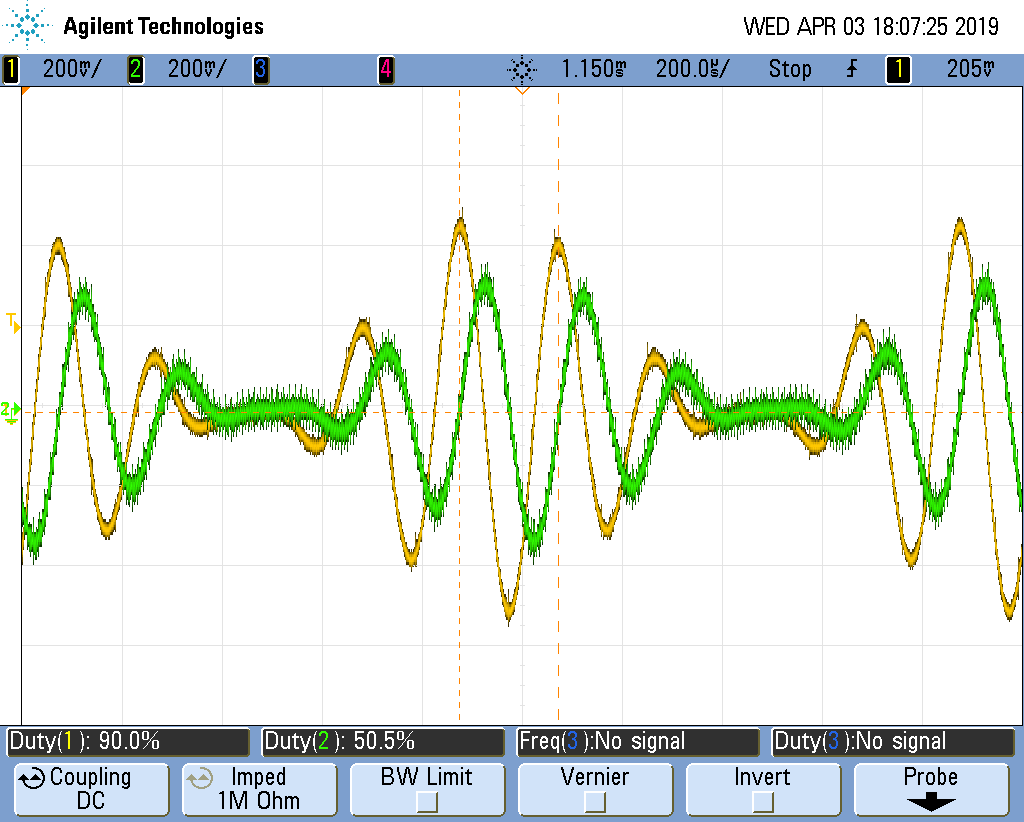
\includegraphics[width=0.45\textwidth]{figures/lyh_pto_7_3.png}}
\caption{Remuestreo de la se\~nal con sample and hold y llave analógica, despues del filtro recuperador}
\end{figure}

\begin{figure}[H]
\centering
\subcaptionbox{Simulacion}
{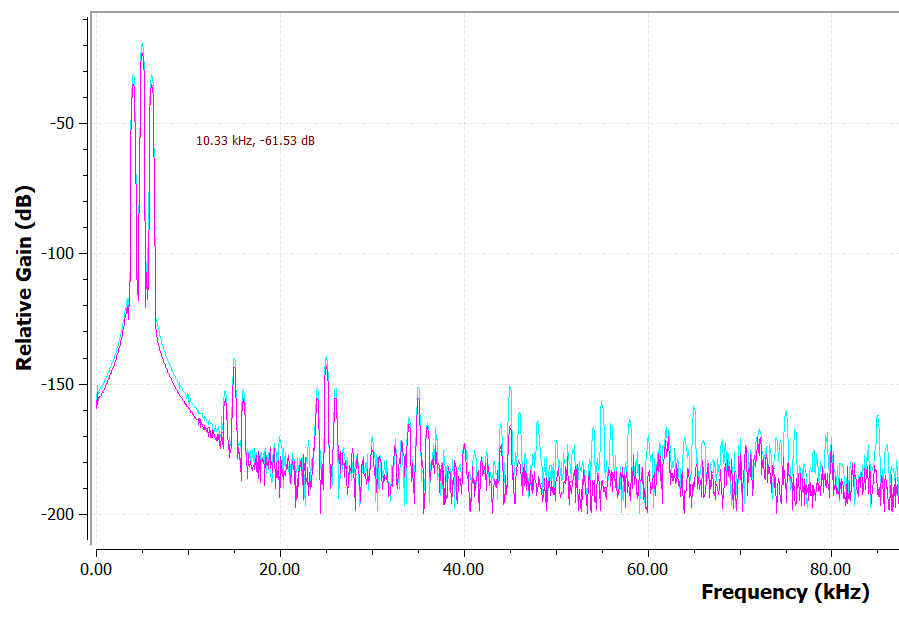
\includegraphics[width=0.5\textwidth]{figures/llsyhsimesp.PNG}}
\subcaptionbox{Medicion}
{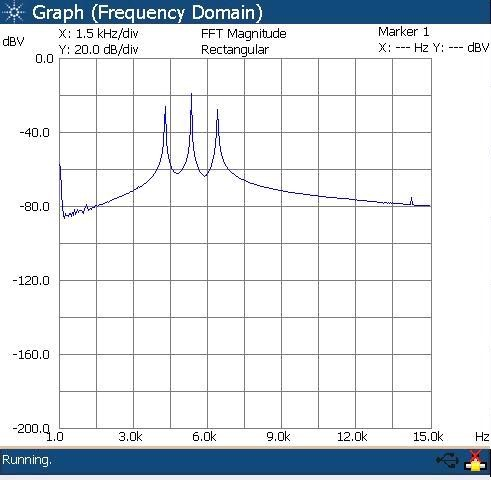
\includegraphics[width=0.45\textwidth]{figures/syh_llave.jpeg}}
\caption{Espectro de la se\~nal despues del sample and hold}
\end{figure}

\end{document}
